\section{Numerical experiments}
\label{sec:numerical_experiments}

\subsection{Implementation}%
\label{sec:implementation_details}

The finite element forward models were implemented in \texttt{C++} and make use of the finite element library \texttt{deal.ii} \cite{dealII93}.

\todo{
All surface and volume integral operators are discretized with Gaussian quadrature using $p_{\text{order}}+1$ one-dimensional (1D) quadrature points in each spatial direction, where $p_{\text{order}}$ is the polynomial order of the finite element space (space)}. 
%$W_h^\porder$.

Convergence results are reported using the relative $L^2$-errors 
\begin{equation}
  \erroru(t) = \frac{ \left\lVert \vel(\bm{x}, t) - \velh(\bm{x}, t)\right\rVert_{\LII(\dom_h)} }{ \left\lVert \vel(\bm{x}, t) \right\rVert_{\LII(\dom_h)} }, \qquad 
  \errorp(t) =\frac{ \left\lVert \p(\bm{x}, t) - \ph(\bm{x}, t)\right\rVert_{\LII(\dom_h)} }{ \left\lVert \p(\bm{x}, t) \right\rVert_{\LII(\dom_h)} },
\end{equation}
where each of the $\LII$-norms over the computational domain $\dom_h$ is calculated using Gaussian quadrature over the element volumes using $p_{\bm{u}} + 3$ for errors in the velocity and $p_{p} + 3$ for errors in the pressure variables.
Unless explicitly specified, the abbreviations $\erroru$ and $\errorp$ refer to the velocity and pressure errors at the final time $T$.


\subsection{On the solution of the pure Neumann problem}

In the case of pure Dirichlet boundaries on the velocity predictor, the pressure level is undefined. 
To see this, note that if the scalar field $\delta p_h$ is a solution of (\ref{eq:PC_presure_poisson}) with $\Gamma_N = \partial \Omega$, then $\delta p_h + c$ for any $c \in \reals$ is also a solution. 
Discretely, the null space of the linear system arising due to the discretization of (\ref{eq:PC_presure_poisson}) is spanned by the set of constant vectors, implying a singular linear system.


Although crucial to the performance of pressure correction schemes, the issue of finding a solution to the singular system in such cases receives little attention in the literature. 
iterative solvers \cite{axelsson_iterative_1996,iankov_finite_2013}, 
An approach favored by many practitioners is to manually specify the value of the candidate solution at a single point by removing an equation from the discrete system and applying a Dirichlet constraint fixing the value of the solution at that point to an arbitrary constant, eliminating the null space and allowing solution of the linear system using a conventional direct solver.
However, in a finite-element context, the function $\delta_p$ is often represented in the Sobolev space $H^1(\Omega)$ or $L^2(\Omega)$, spaces in which point evaluations do not make sense. 
In these cases, imposing such a constraint can render the variational problem ill-posed.

\todo{
This is complicated by the fact that some numerical linear algebra software varies widely in terms of implementation; while some libraries will not solve a singular system (numpy), other direct procedures will do so when they can identify a zero-pivot. 
Similar for iterative solvers.}


In \cite{bochev_finite_2005}, the authors rigorously describe strategies for addressing the singular system in a continuous finite element context. 
Here, we extend that discussion to the DG-FEM setting and illustrate computational trade-offs associated with some candidate approaches.

As a first approach, we apply a subspace projection using a Krylov-solver \cite{vorst_iterative_2003}, making use of the fact that iterative solvers solve singular systems provided that the right-hand side is in the orthogonal complement of the null-space.
\todo{
This modification is ok because we're only removing the null space contribution to the linear system
}
As a second approach, we apply a penalty-based method which can be interpreted as a regularization.
This method, while simple and independent of linear solver type, involves the specification of a hyperparameter $\gamma$.
As a third approach, we impose a mean-value constraint 
\begin{equation}
  \int_{\Omega}^{} \delta p \,d\Omega = 0
  \label{eq:mean_value_zero_condition}
\end{equation}
into the linear system directly, avoiding the saddle point system that arises as a result of applying the constraint as a Lagrange multiplier \cite{bochev_finite_2005}.

\todo{
As a test case, we use a manufactured solution
How to do the zero-mean removal?
}

Boundary conditions and forcing function are deduced from the exact solution
\begin{equation}
    \delta_p^* = \frac{1}{3} \sin\left(-\frac{\pi}{2} x \right) \cos\left(2\pi y\right).
\end{equation}
We consider the domain $\Omega = [-1, 1]^2$, and by symmetry, we have that the exact solution $\delta_p^*$ is analytically zero-mean in the sense of equation (\ref{eq:mean_value_zero_condition}).

\begin{figure}[htpb]
  \centering
  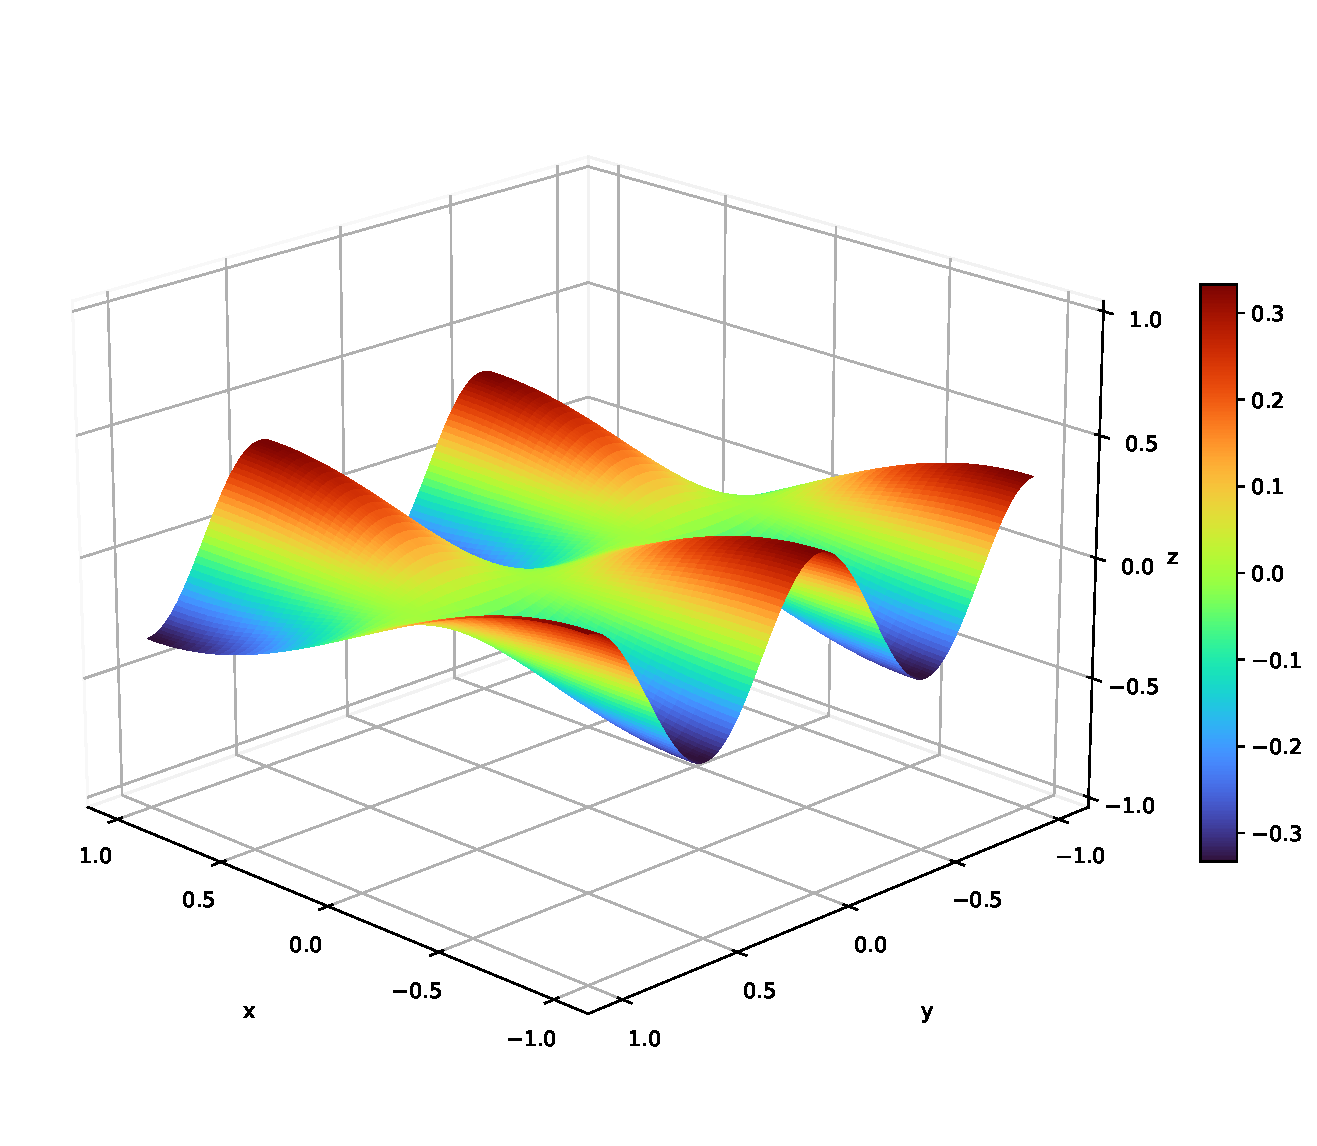
\includegraphics[width=0.5\linewidth]{img/dp_study_analytical.pdf}
  \caption{Analytical solution of the pure Neumann problem}
  \label{fig:dp_neumann_problem_analytical}
\end{figure}




\subsection{Unsteady Stokes Flow}

The review paper \cite{guermond_overview_2006} solves the unsteady Stokes problem

\begin{equation}
  \begin{aligned}
    \bm{u}(\bm{x}, t) &= \pi \sin t 
    \begin{pmatrix}
      \sin( 2\pi y) \sin^2( \pi x) \\
      -\sin(2 \pi x) \sin^2(\pi y)
    \end{pmatrix} \\
    p(\bm{x}, t) &= \sin(t)\cos(\pi x) \sin(\pi y)\\
  \end{aligned}
  \label{eq:MS_stokes_guermond}
\end{equation}
where the source term $f= u_t -\nu \nabla \cdot( \nabla \bm{u} ) + \nabla p $.

In \cite{fehn_stability_2017}, we have
\begin{equation}
  \begin{aligned}
  \bm{u}(\bm{x}, t) &= 
  \begin{pmatrix}
    \sin(x) (a\sin(a y) - \cos(a)\sinh(y)) \\
    \cos(x) (\cos(a y) + \cos(a)\cosh(y))
  \end{pmatrix}
  \exp(-\lambda t),\\
    p(\bm{x}, t) &= \lambda \cos(a) \cos(x) \sinh(y) \exp(-\lambda t)
  \end{aligned}
  \label{eq:MS_unsteady_stokes_fehn}
\end{equation}
where $\lambda = \nu(1 + a^2)$ $\nu = 1$ and $a = 2.883356$ on a domain of  $\Omega = [-1, 1]^2$; they take $[0, T] = [0, 0.1]$ and Dirichlet boundary conditions everywhere, $\Gamma = \Gamma_D$.

\subsection{Verification}
Spatial convergence test, temporal convergence test




\subsection{Taylor-Green vortex flow}
Is this the same test case as in Hesthaven?

\subsection{Backward facing step}

\subsection{Lid-driven cavity flow}

\subsection{Lock Exchange?}
\subsection{Lab RTI flow?}
